\subsection{Test af programmet}
\label{sec:test}

Som en del af problemløsningen udføres der test på det udviklede program. Formålet med testafsnittet er at undersøge om programmet lever op til de programkrav som blev opstillet i slutningen af teoriafsnit, \ref{sec:teori}. Testene vil være med til at belyse eventuelle fejl og mangler i programmet.

Først testes det om programmet kan rendere et billede af en lampe og dens belysning. Dette gøres ved at sammenligne et billede taget med et fysisk kamera, med et billede renderet af programmet.

Figuren herunder viser forsøgsopstillingen.


Figur \ref{fig:test_real_fake} herunder viser billedet taget med et mobilkamera(Samsung Galaxy S3) og billedet renderet af programmet med nedenstående input.
\begin{lstlisting}
./trace model.ply -V 0.785 -t 2700 -w 540 -h 960
\end{lstlisting}

\begin{figure}[H]
\centering
\begin{subfigure}{.5\textwidth}
  \centering
  \includegraphics[width=.4\linewidth]{real}
  \caption{}
  \label{fig:real}
\end{subfigure}%
\begin{subfigure}{.5\textwidth}
  \centering
  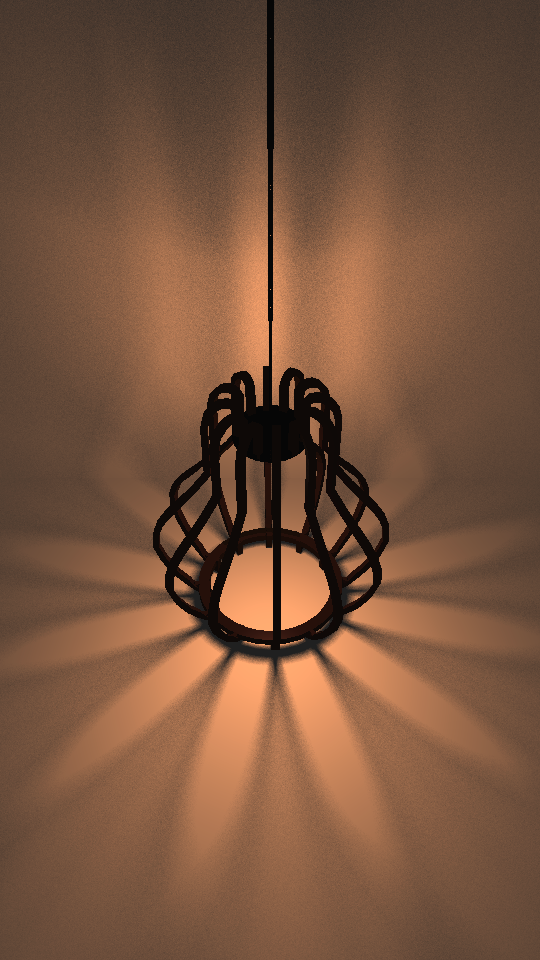
\includegraphics[width=.4\linewidth]{result_5305s}
  \caption{}
  \label{fig:fake}
\end{subfigure}
\caption{Viser billede taget med mobilkamera (a) og billede renderet af programmet (b). For de to billeder gælder at pærens farvetemperatur er 2700K.}
\label{fig:test_real_fake}
\end{figure}

For at teste de forskellige brugerinput, som kan indtastes i programmet, er der herunder billeder med forskellige brugerinput.

Først testes farvetemperaturen.
\begin{figure}[H]
\centering
\begin{subfigure}{.5\textwidth}
  \centering
  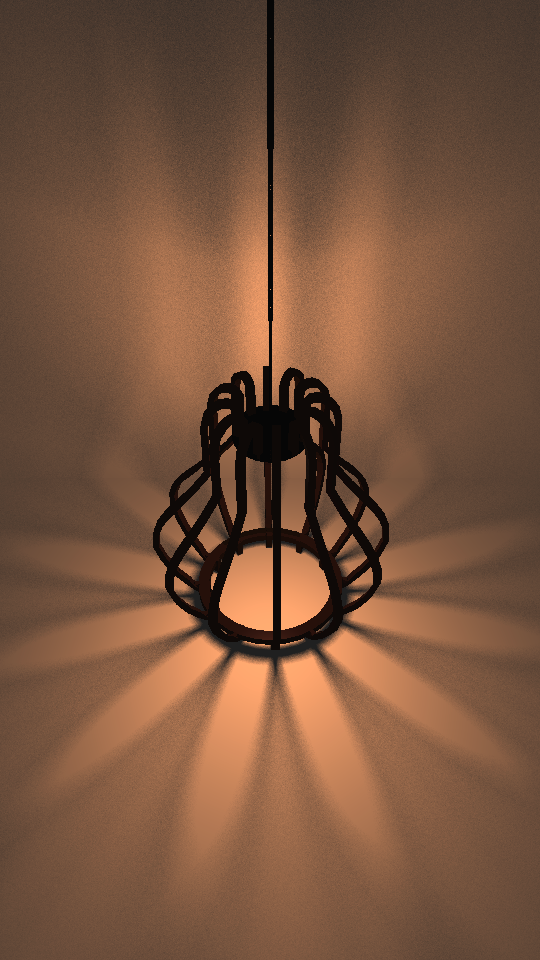
\includegraphics[width=.4\linewidth]{result_5305s}
  \caption{}
  \label{fig:real}
\end{subfigure}%
\begin{subfigure}{.5\textwidth}
  \centering
  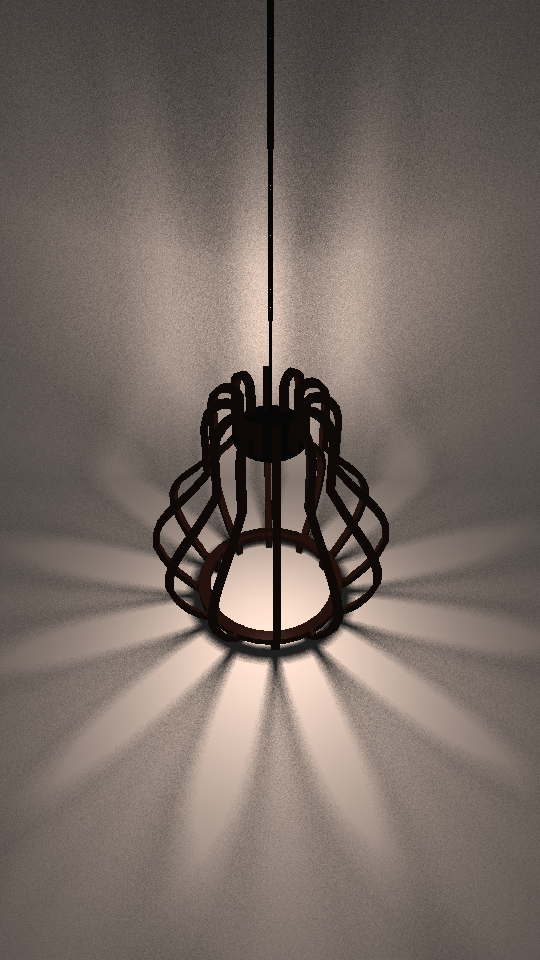
\includegraphics[width=.4\linewidth]{result_2734s_5000k_0H_0-785V}
  \caption{}
  \label{fig:fake}
\end{subfigure}
\caption{Viser billede renderet af programmet, med farvetemperaturer på 2700K (a) og 5000K (b).}
\label{fig:farvetemp}
\end{figure}

Herefter sammenlignes billeder renderet med forskellige vinkler.
\begin{figure}[H]
\centering
\begin{subfigure}{.5\textwidth}
  \centering
  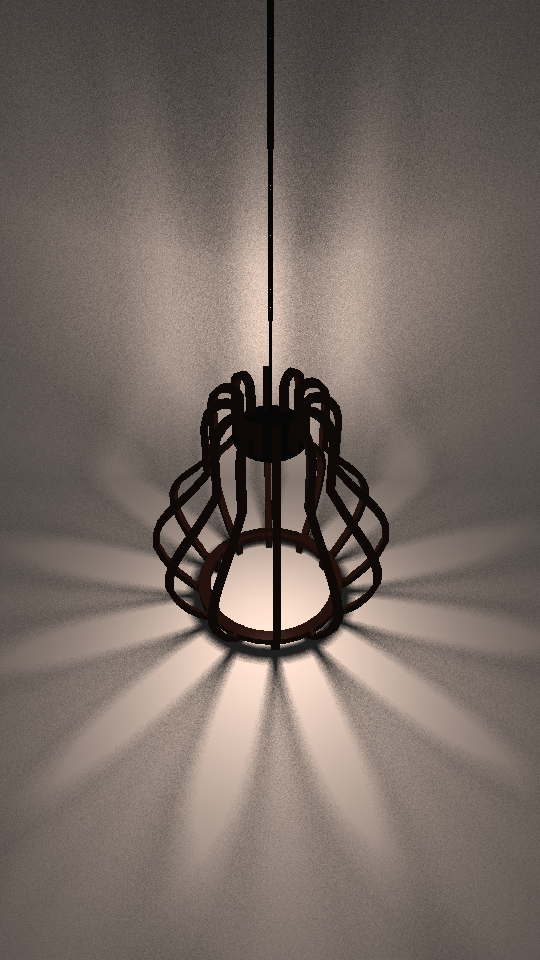
\includegraphics[width=.4\linewidth]{result_2734s_5000k_0H_0-785V}
  \caption{}
  \label{fig:real}
\end{subfigure}%
\begin{subfigure}{.5\textwidth}
  \centering
  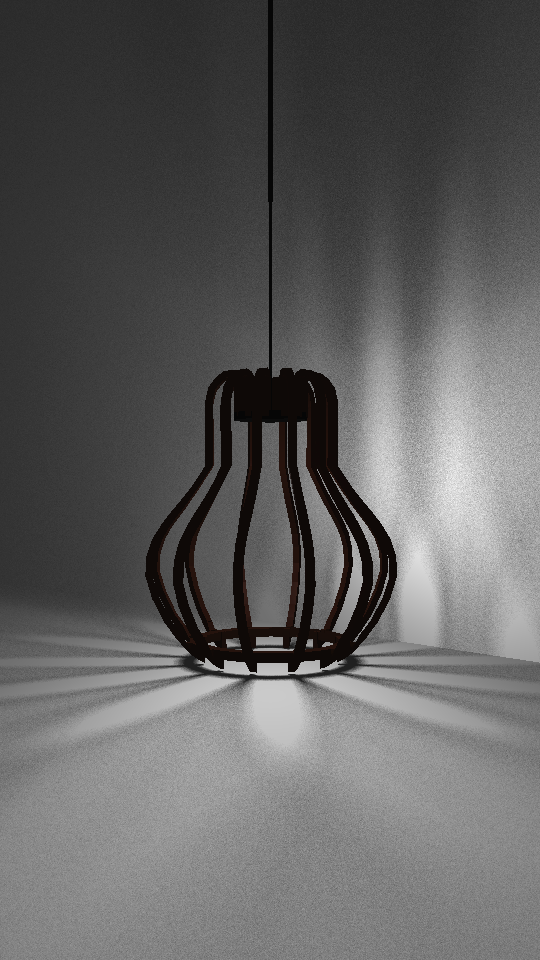
\includegraphics[width=.4\linewidth]{result_2758s_white_0-8H}
  \caption{}
  \label{fig:fake}
\end{subfigure}
\caption{Viser billede renderet af programmet, med vinkler 0H 0.785V (a) og 0.8H 0V (b).}
\label{fig:synsvinkel1}
\end{figure}

\begin{figure}[H]
\centering
\begin{subfigure}{.5\textwidth}
  \centering
  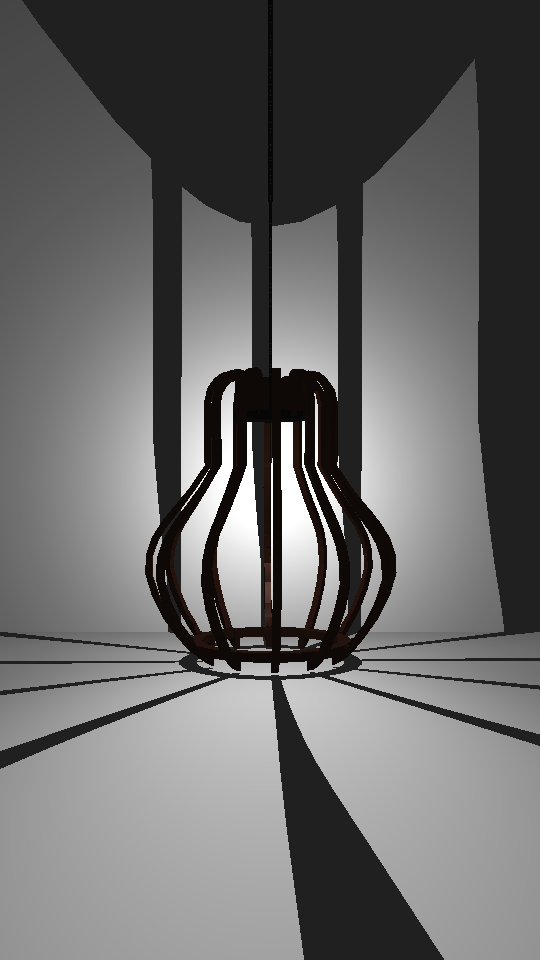
\includegraphics[width=.4\linewidth]{result_1sample_white_57s}
  \caption{}
  \label{fig:real}
\end{subfigure}%
\begin{subfigure}{.5\textwidth}
  \centering
  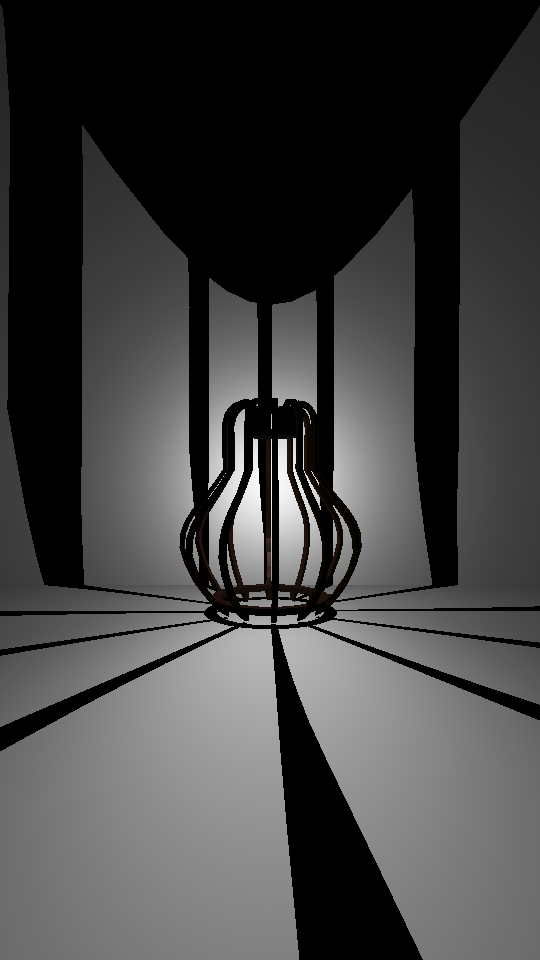
\includegraphics[width=.4\linewidth]{result_1sample_white_old_523s}
  \caption{}
  \label{fig:fake}
\end{subfigure}
\caption{Viser billede renderet af programmet, med tider 57 Sek[Ny algo] (a) og 523 Sek[Gamel algo med bounding spheres] (b). Billederne er forskællige fordi den gamle algoritme udregner synsvinklen på en anden måde}
\label{fig:synsvinkel1}
\end{figure}

\subsection*{Opsummering}
Som vist på figur \ref{fig:fake} opfylder programmet krav 1-3 fra afsnit \ref{sec:krav_til_kode}, da den kan rendere og gemme et billede af en lampe og dens belysning på baggrund af indtastede input der indeholder 3D-fil, farvetemperatur, synsvinkel og opløsningen af billedet. Derudover er der som vist sket en optimering af programmets renderingstid efter implementeringen af kd-træer. 
Som det er vist på figur \ref{fig:test_real_fake} er der en afvigelse mellem billedet af den rigtige lampe og det renderede billede af en model af lampen. Denne afvigelse diskuteres i næste afsnit sammen med rapportens resterende resultater. 

%Der er nu blevet udført forskellige test af programmet, som senere diskuteres i afsnit \ref{sec:diskussion}.